

\setkeys{Gin}{width=\textwidth}

\subsection{Simple (semi-artificial!) Example: logit(exp(-L))}
\begin{frame}[fragile]
  Logistic regression: Computing ``logit()''s, $\log \frac{p}{1-p}$
  accurately for very small $p$, i.e., $p = \exp(-L)$, or
  \vspace*{-.6ex}
  \[
  \log\frac{p}{1-p} = \log p - \log(1 - p) = -L - \log(1 - \exp(-L)),
  \]
  \vspace*{-.5ex}

  and hence $-\log(1 - \exp(-L))$ is needed, e.g.,
  when p is really really close to 0, say $p = 10^{-1000}$, as then
  we can only compute $\logit(p)$, if we specify  $L := -\log(p) \leftrightarrow p = \exp(-L)$.

\begin{Schunk}
\begin{Sinput}
> curve(-log(1 - exp(-x)), 0, 10)
\end{Sinput}
\end{Schunk}
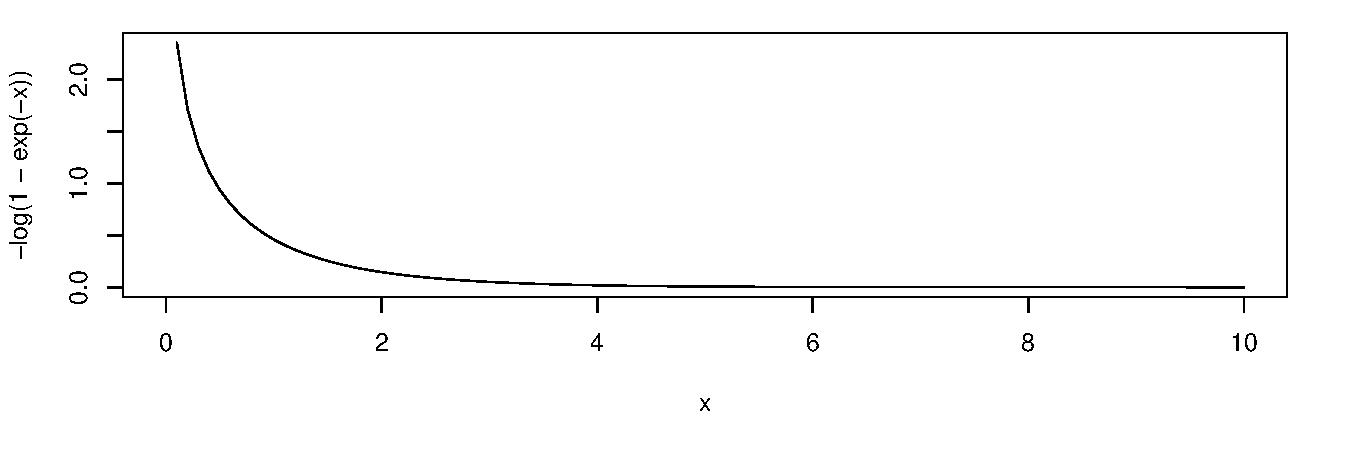
\includegraphics{log1exp-log1-exp-curve-10}

seems fine. --- ---  However, \dots
\end{frame}

\begin{frame}[fragile]
However, further out to 50 (and on a log scale), we observe

\begin{Schunk}
\begin{Sinput}
> curve(-log(1 - exp(-x)),  0, 50, log="y")
\end{Sinput}
\end{Schunk}
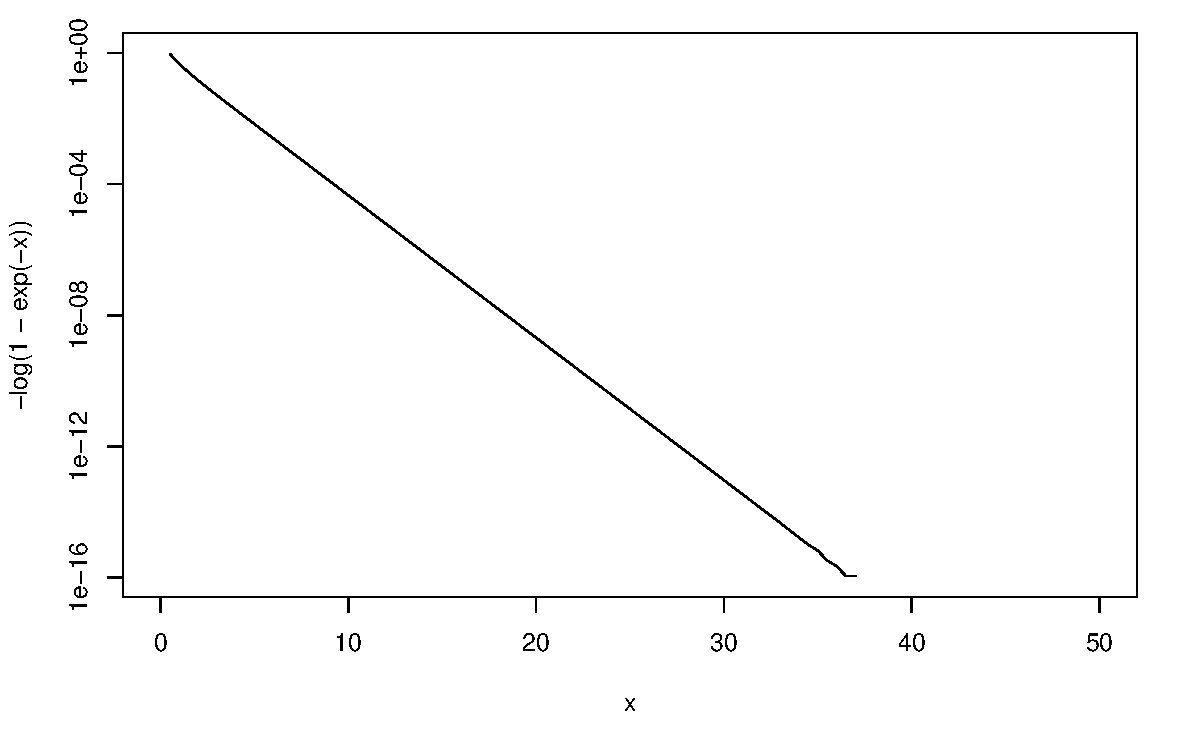
\includegraphics{log1exp-log1-exp-curve-log}
\\[-.6ex]
which shows early underflow.
\end{frame}

\begin{frame}[fragile]
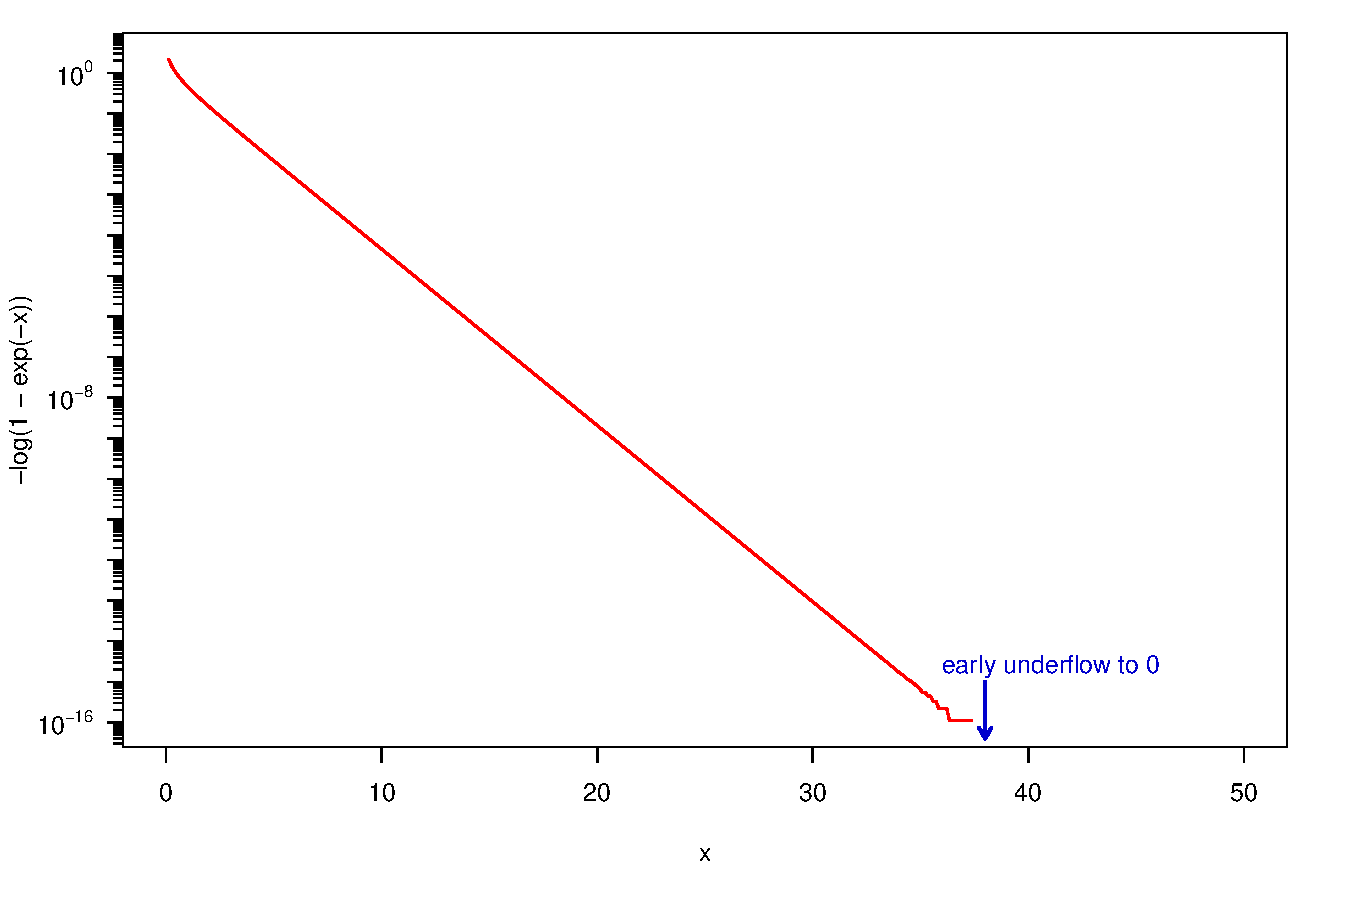
\includegraphics{log1exp-log1-exp-log-niceer}
\end{frame}

\begin{frame}[fragile]
What did happen?  Look at
\begin{Schunk}
\begin{Sinput}
> x <- -40:-35
>     -log(1 - exp(x))
\end{Sinput}
\begin{Soutput}
[1] 0.000000e+00 0.000000e+00 0.000000e+00 1.110223e-16 2.220446e-16
[6] 6.661338e-16
\end{Soutput}
\begin{Sinput}
> log(-log(1 - exp(x)))# --> -Inf values
\end{Sinput}
\begin{Soutput}
[1]      -Inf      -Inf      -Inf -36.73680 -36.04365 -34.94504
\end{Soutput}
\begin{Sinput}
> ## ok, how about more accuracy
> x. <- mpfr(x, 120)
> log(-log(1 - exp(x.)))# aha... looks perfect now
\end{Sinput}
\begin{Soutput}
6 'mpfr' numbers of precision  120   bits 
[1] -39.999999999999999997932904877538241734
[2]  -38.99999999999999999423372196756935807
[3]  -37.99999999999999998430451715981029611
[4] -36.999999999999999957331848579613165434
[5] -35.999999999999999884024061830552087239
[6] -34.999999999999999684744214015307532692
\end{Soutput}
\end{Schunk}
\end{frame}

\begin{frame}[fragile]
And visually:
\begin{Schunk}
\begin{Sinput}
> x <- seq(-40, -20, by = .5)
> plot(x,x, type="n", ylab="", ann=FALSE)
> lines(x, log(-log(1 - exp(x))), type = "o", col = "purple", lwd=3, cex = .6)
\end{Sinput}
\end{Schunk}
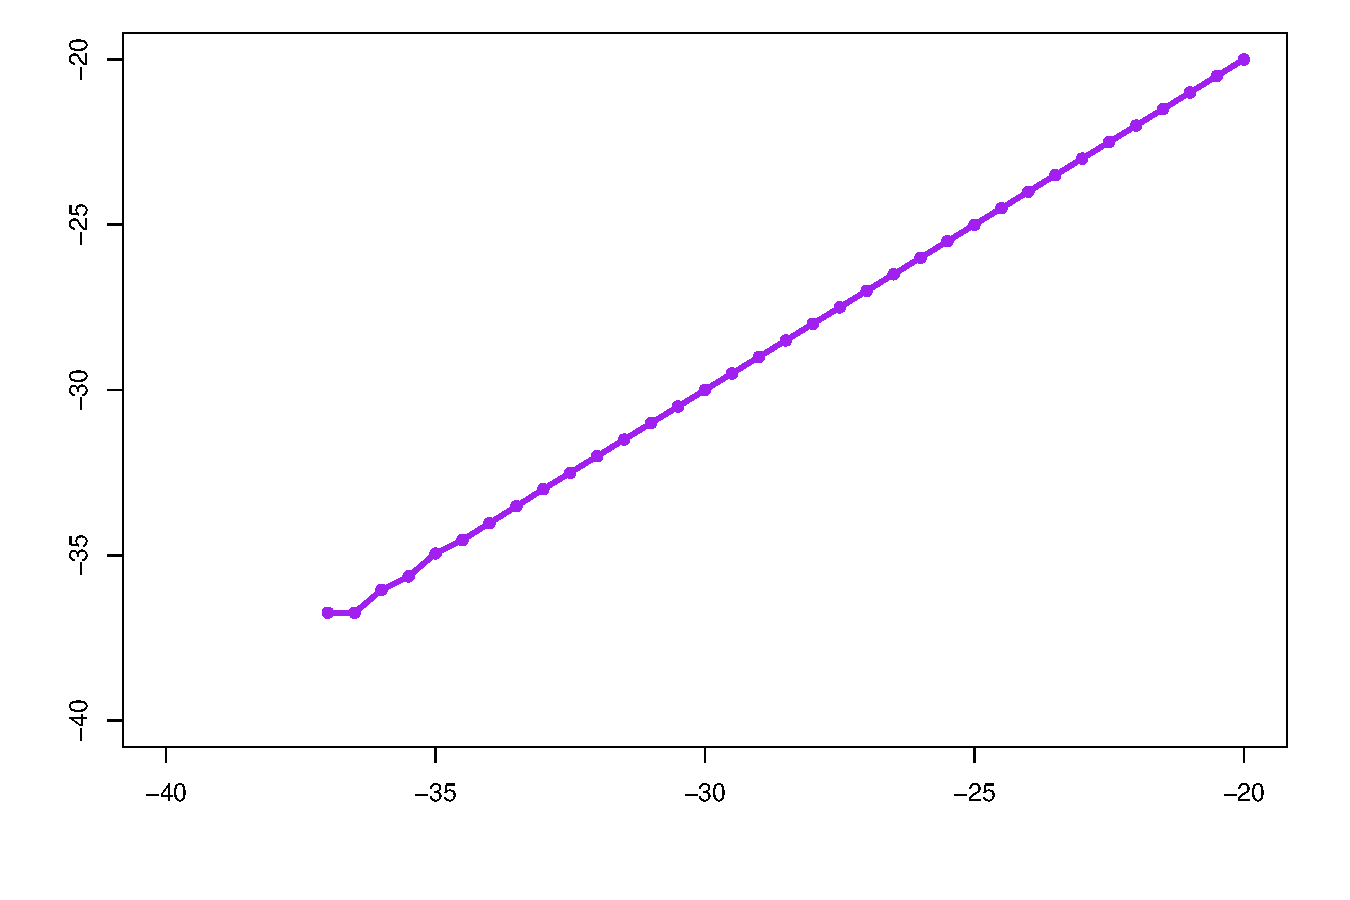
\includegraphics{log1exp-plot-log1exp-ex}
\end{frame}

\begin{frame}[fragile]
Now repeat this with ``with accuracy'':
\begin{Schunk}
\begin{Sinput}
> x <- seq(-40, -20, by = .5)
> plot(x,x, type="n", ylab="", ann=FALSE)
> lines(x, log(-log(1 - exp(x))), type = "o", col = "purple", lwd=3, cex = .6)
> x. <- mpfr(x, 120)
> lines(x, log(-log(1 - exp(x.))), col=2, lwd=1.5)
\end{Sinput}
\end{Schunk}
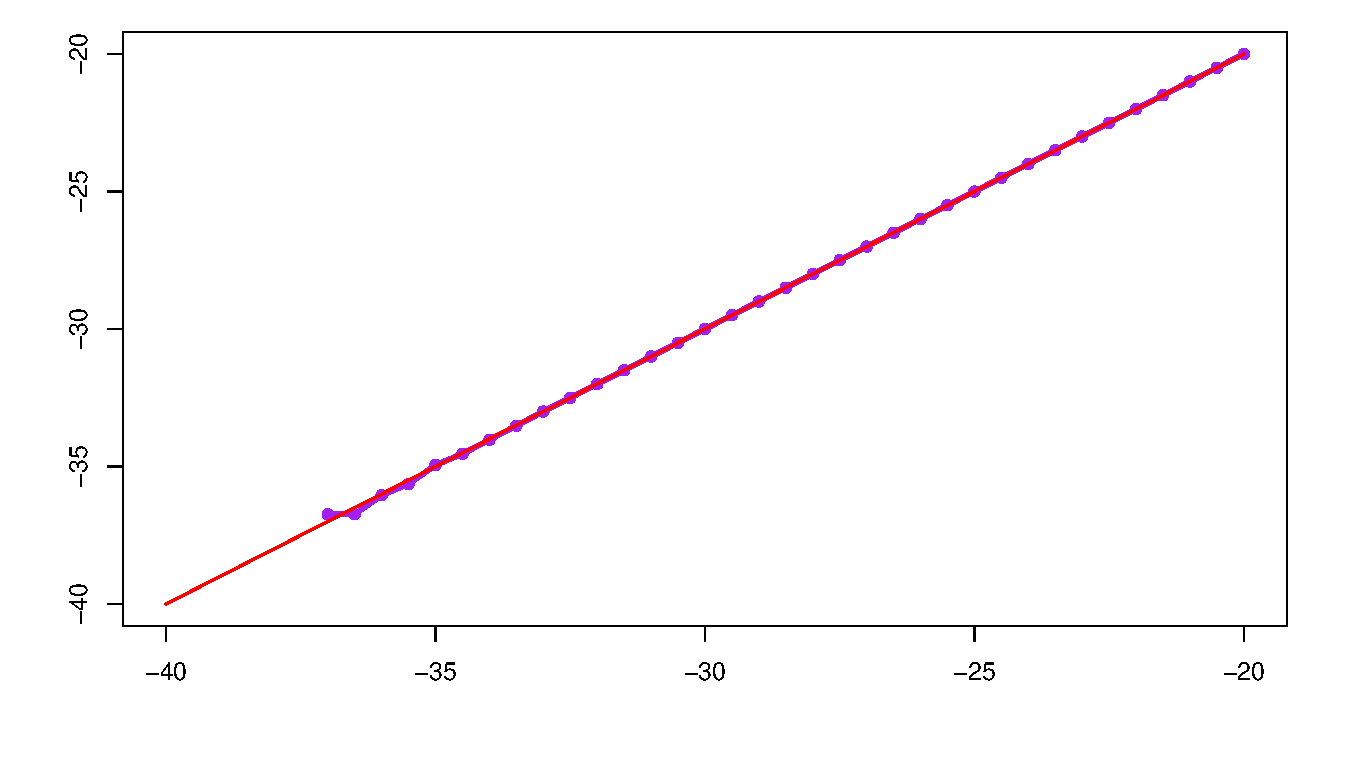
\includegraphics{log1exp-plot-log1exp-mpfr}
\end{frame}


%%% Local Variables:
%%% TeX-command-default: "LaTeX PDF"
%%% TeX-master: "Maechler_Rmpfr.tex"
%%% End:

